\documentclass[a4paper]{article}

\usepackage[english]{babel}
\usepackage[utf8]{inputenc}
\usepackage{amsmath}
\usepackage{graphicx}
\usepackage{float}
\usepackage[colorinlistoftodos]{todonotes}
\usepackage{listings}
\usepackage{color}
\usepackage[margin=1in]{geometry}

\definecolor{mygreen}{rgb}{0,0.6,0}
\definecolor{mygray}{rgb}{0.5,0.5,0.5}
\definecolor{mymauve}{rgb}{0.58,0,0.82}

%% Source Code Design
\lstnewenvironment{MATLAB}{
\lstset{ %
  backgroundcolor=\color{white},   % choose the background color; you must add \usepackage{color} or \usepackage{xcolor}
  basicstyle=\footnotesize,        % the size of the fonts that are used for the code
  breakatwhitespace=false,         % sets if automatic breaks should only happen at whitespace
  breaklines=true,                 % sets automatic line breaking
  captionpos=b,                    % sets the caption-position to bottom
  commentstyle=\color{mygreen},    % comment style
  deletekeywords={...},            % if you want to delete keywords from the given language
  escapeinside={\%*}{*)},          % if you want to add LaTeX within your code
  extendedchars=true,              % lets you use non-ASCII characters; for 8-bits encodings only, does not work with UTF-8
  frame=single,                    % adds a frame around the code
  keepspaces=true,                 % keeps spaces in text, useful for keeping indentation of code (possibly needs columns=flexible)
  keywordstyle=\color{blue},       % keyword style
  language=Matlab,                 % the language of the code
  morekeywords={*,...},            % if you want to add more keywords to the set
  numbers=none,                    % where to put the line-numbers; possible values are (none, left, right)
  numbersep=5pt,                   % how far the line-numbers are from the code
  numberstyle=\tiny\color{mygray}, % the style that is used for the line-numbers
  rulecolor=\color{black},         % if not set, the frame-color may be changed on line-breaks within not-black text (e.g. comments (green here))
  showspaces=false,                % show spaces everywhere adding particular underscores; it overrides 'showstringspaces'
  showstringspaces=false,          % underline spaces within strings only
  showtabs=false,                  % show tabs within strings adding particular underscores
  stepnumber=2,                    % the step between two line-numbers. If it's 1, each line will be numbered
  stringstyle=\color{mymauve},     % string literal style
  tabsize=4,                       % sets default tabsize to 2 spaces
  title=\lstname                   % show the filename of files included with \lstinputlisting; also try caption instead of title
}}{}

\title{ENCM 509 - Laboratory \#1}

\author{Kyle Derby MacInnis - Mebrhatom Aneya}

\date{\today}

\begin{document}
\maketitle

% ABSTRACT
\begin{abstract}
The first lab of this course looked at the basics of loading data and displaying it in MATLAB as well as collecting biometric data from a tablet and using it to look at the statistical distributions of different signature variations.
\end{abstract}

% INTRODUCTION
\section{Introduction}
The lab focuses on signatures as the biometric data of interest, and using a WACOM tablet, ten signatures were collected from both group members and an additional five "forged" signatures were also collected from both members.

The data was collected using an application called SigGet whose main function is to collect and convert the measured information from the tablet and convert into an appropriate \textsc{.mat} file. The parameters of interest which were collected included pressure, position, and time information.

These signatures make up the base of the data being analyzed in this laboratory, and upon the completion  of the collecting process, the lab's next focus was on loading and utilizing the collected data within MATLAB's framework.

Once the data is in a convenient format for MATLAB to process it, performing calculations is easily achieved. For the purpose of this lab, the emphasis was on the collecting process and not on complex calculations. A normal distribution was used as the underlying model to compare the collected data and display it.

% PROCEDURE OF THE LAB
\section{Procedure}
\begin{enumerate}
\item Using SigGet collect 10 separate sets of signature data from each member. Save and store as individual \textsc{.mat} files.
\item Grab an additional 5 sets of "forged" signatures for use later.
\item Using MATLAB and the guidelines in the lab manual, write a script to display the follow:
\begin{itemize}
\item A colour-coded pressure map of the signature data.
\item A colour-coded velocity map of the signature data.
\item A 3D plot of the signature's pressure map.
\item The normal distributions of the velocity data.
\end{itemize}
\item Discuss any noticeable deviations from the expected outcomes, and give some conclusions on the data observed.
\end{enumerate}

% MAIN RESULTS (FIGURES AND TABLES)
\pagebreak
\section{Results}
\begin{enumerate}
\item Pressure Mapped Signatures
	\subsubsection*{Real}
	\begin{figure}[H]
    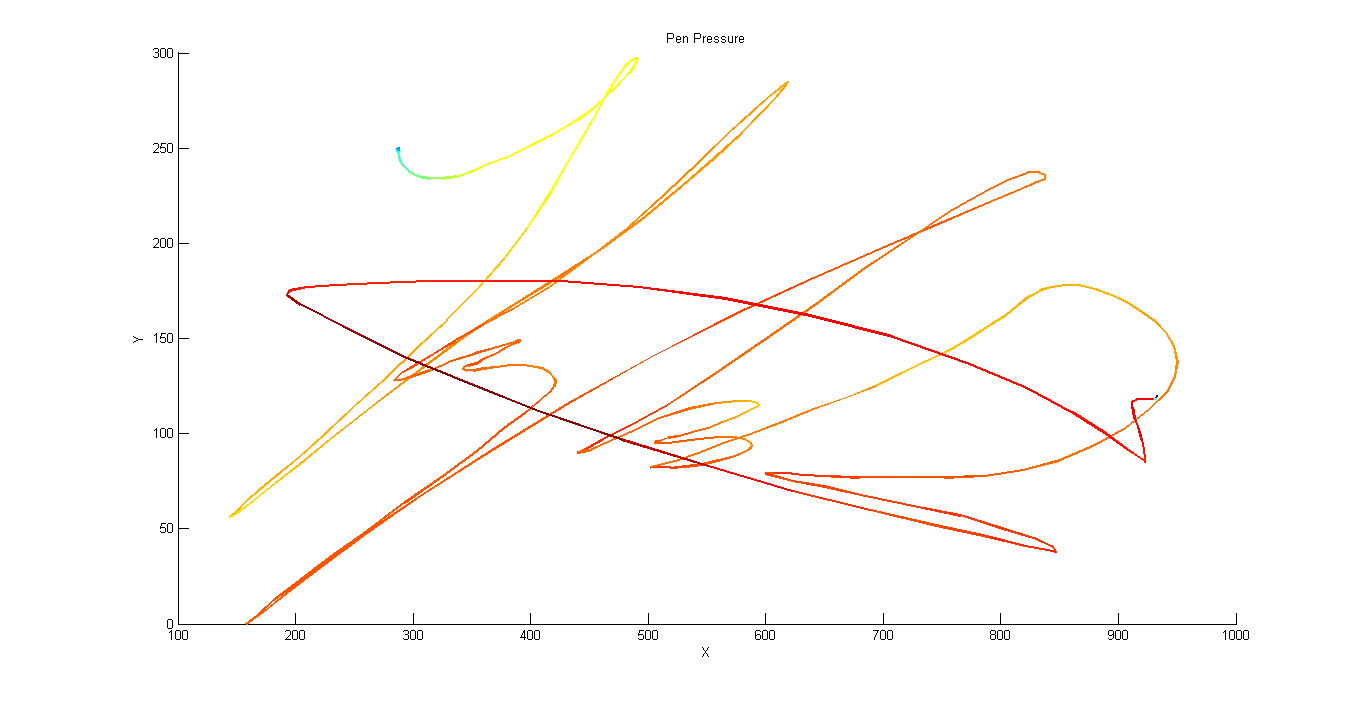
\includegraphics[width=0.5\linewidth]{KSig_Ex_Pressure.png}
    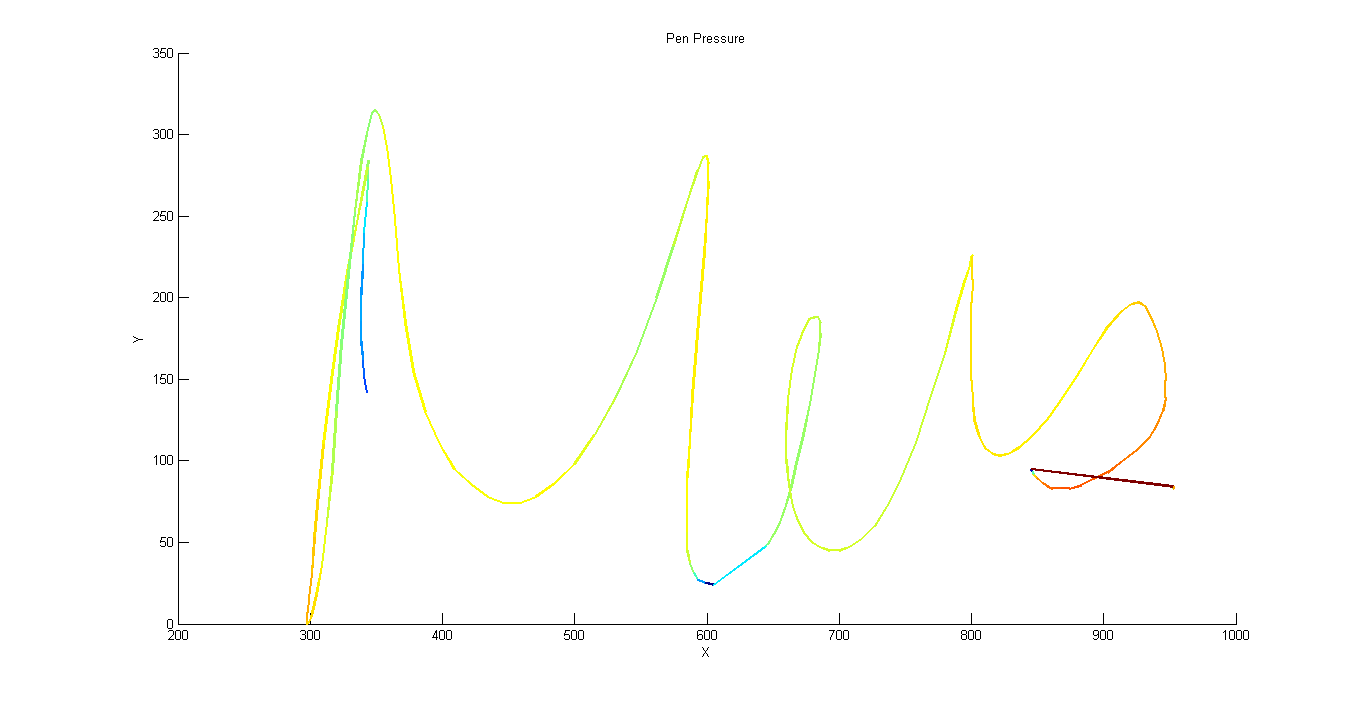
\includegraphics[width=0.5\linewidth]{MSig_Ex_Pressure.png}
    \caption{Example "Real" Pressure Mapped Signatures Captured}
    \end{figure}
    \subsubsection*{Forged}
    \begin{figure}[H]
    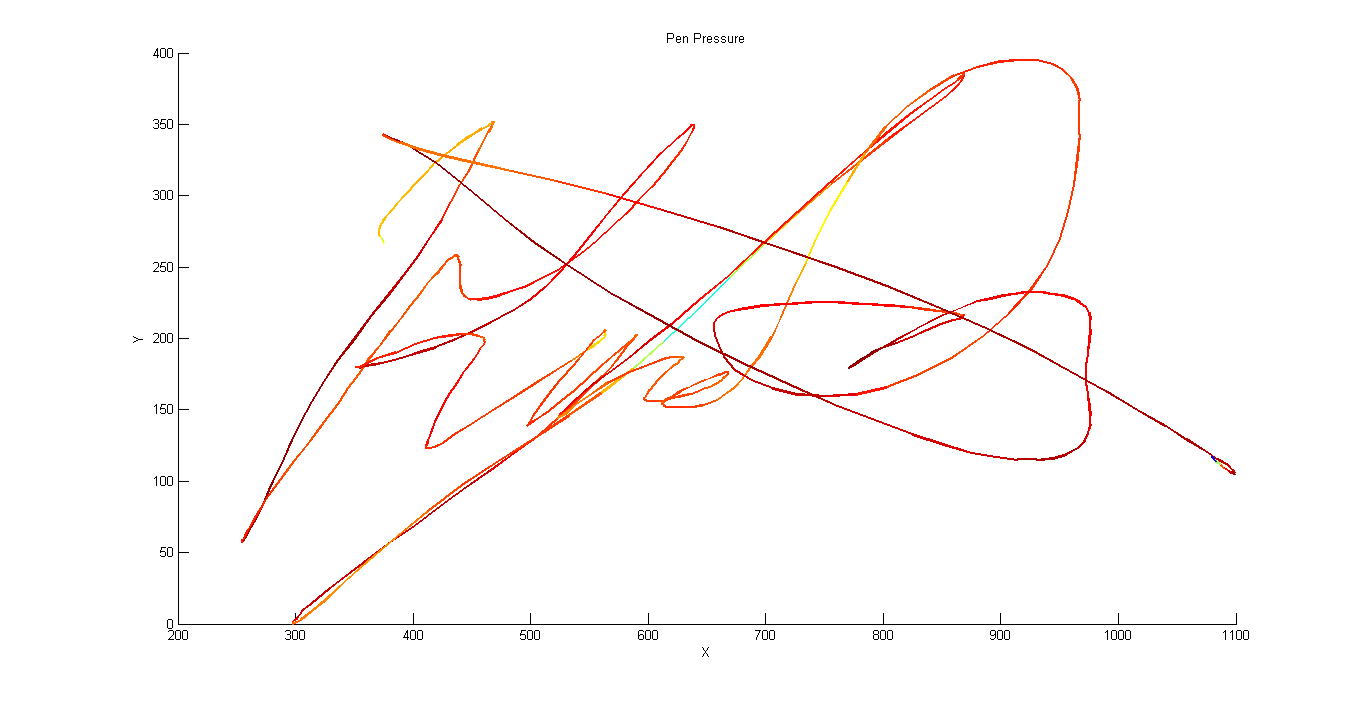
\includegraphics[width=0.5\linewidth]{KSigForge_Pressure.png}
    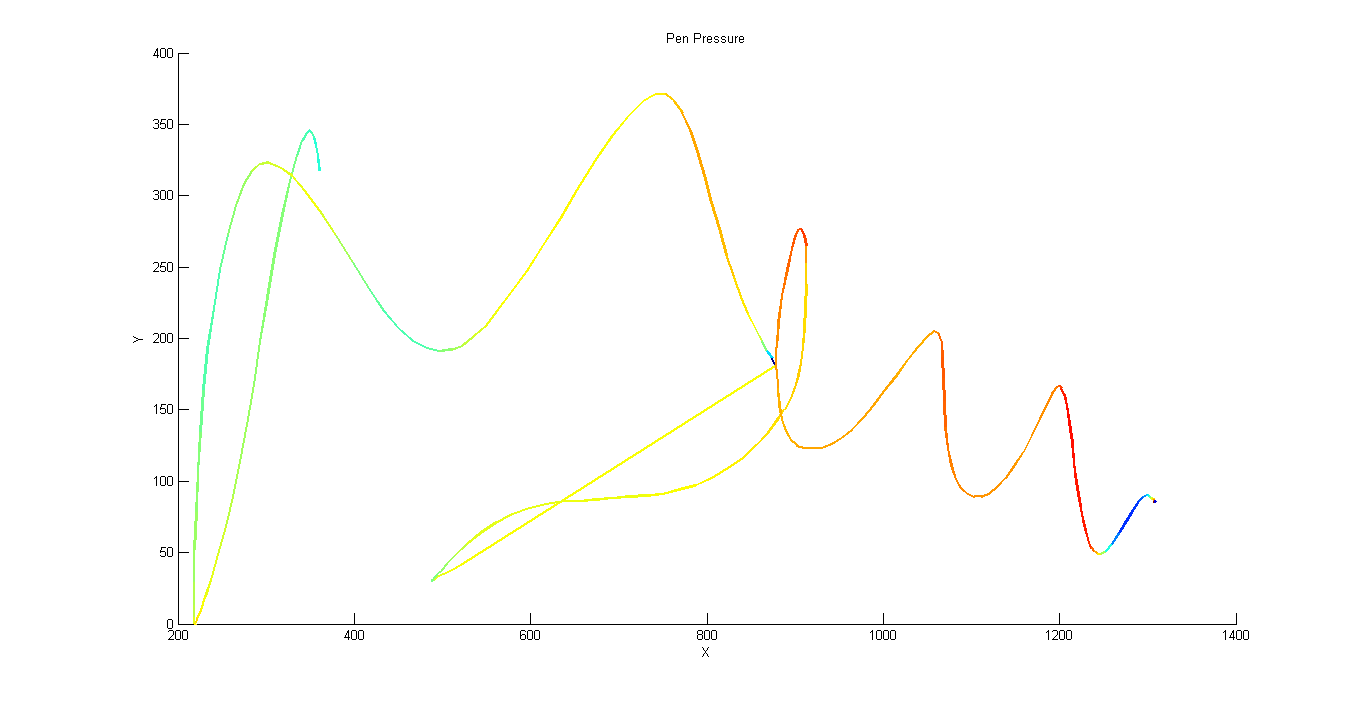
\includegraphics[width=0.5\linewidth]{MSigForge_Pressure.png}
    \caption{Example "Forged" Pressure Mapped Signatures Captured}
    \end{figure}
	% TODO - Screen Capture (A couple Examples)
\item Velocity Mapped Signatures
	\subsubsection*{Real}
    \begin{figure}[H]
    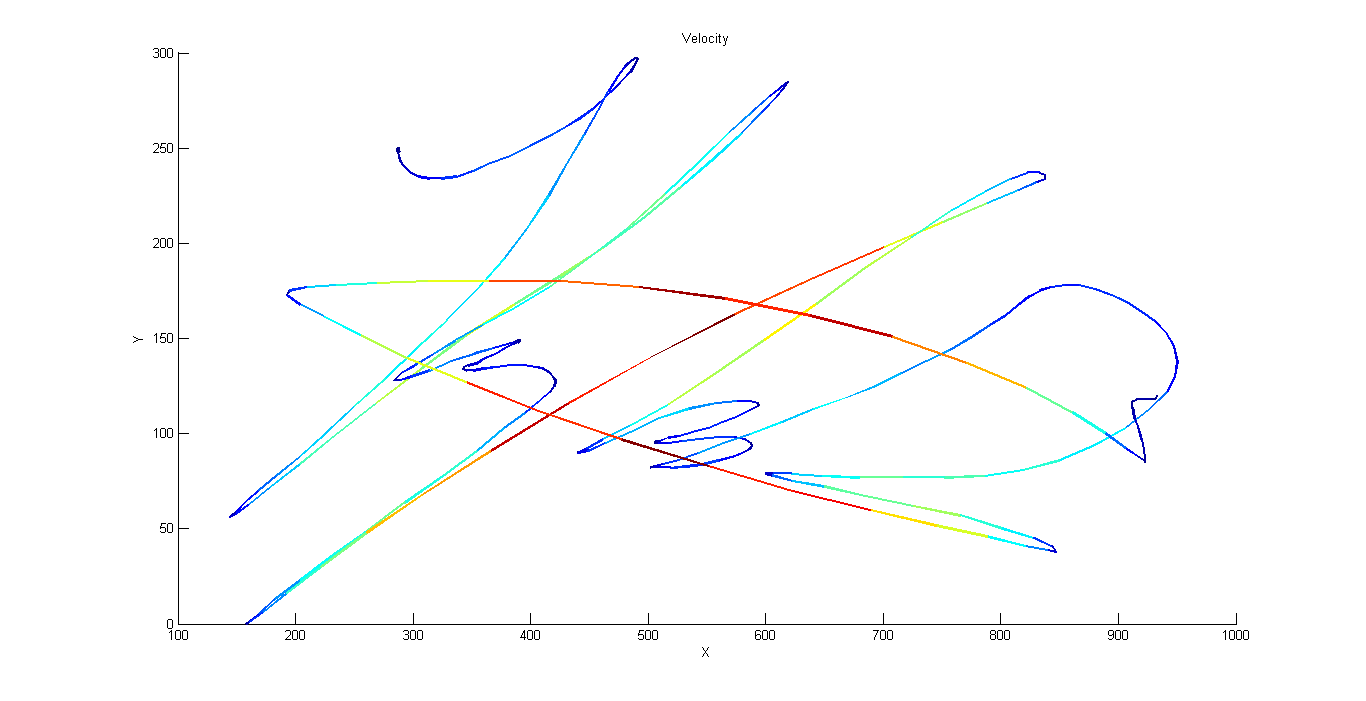
\includegraphics[width=0.5\linewidth]{KSig_Ex_Velocity.png}
    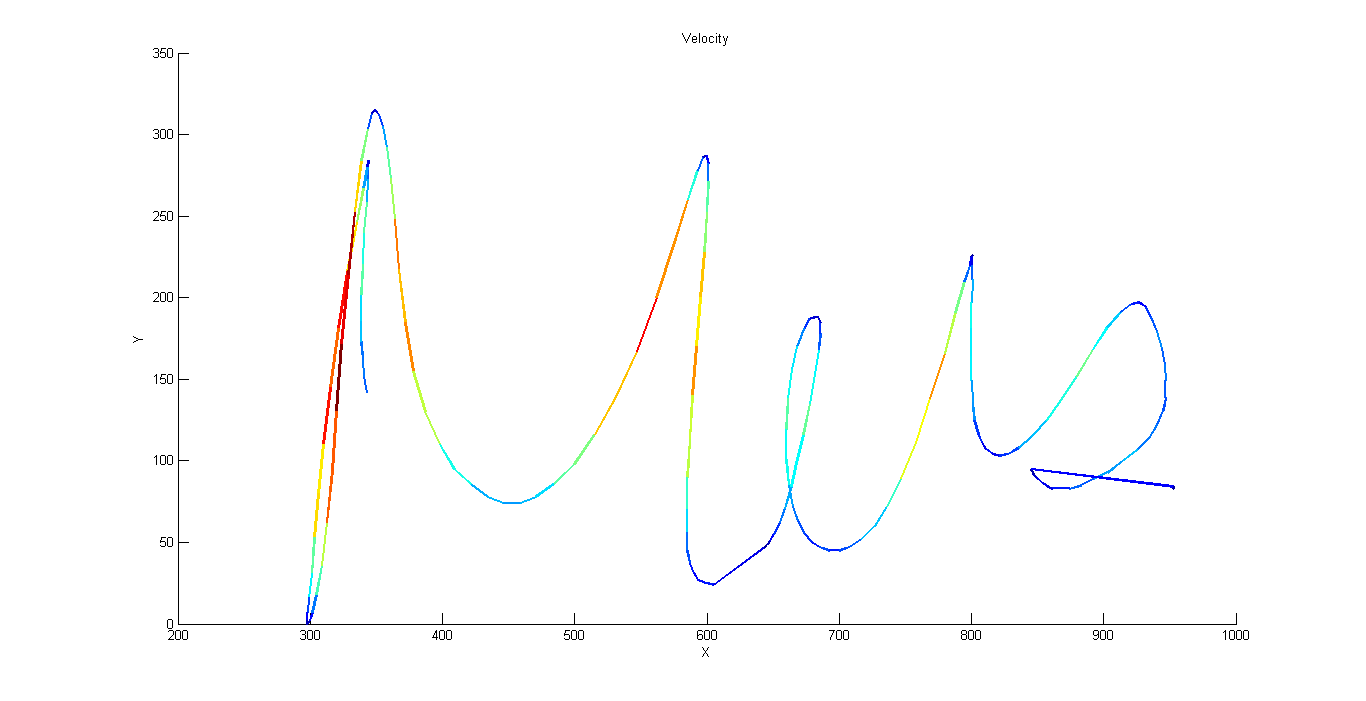
\includegraphics[width=0.5\linewidth]{MSig_Ex_Velocity.png}
    \caption{Example "Real" Velocity Mapped Signatures Captured}
    \end{figure}
    \subsubsection*{Forged}
    \begin{figure}[H]
    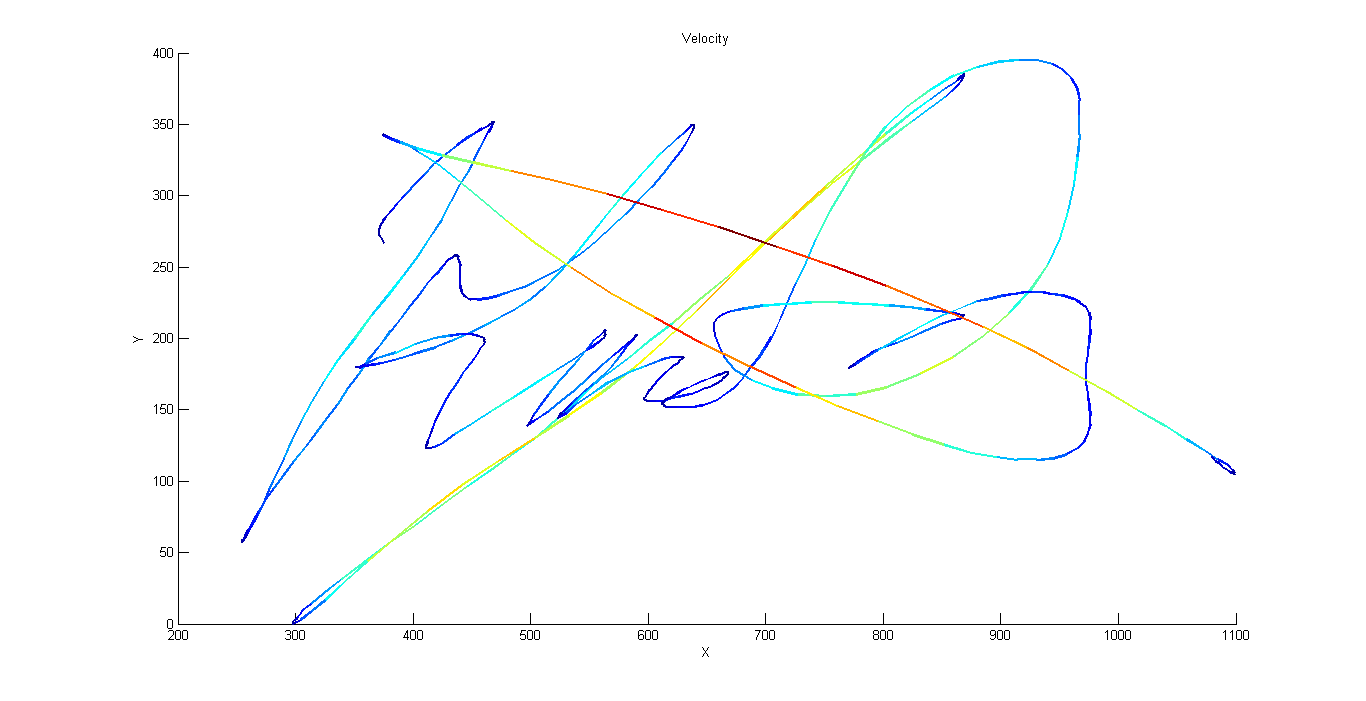
\includegraphics[width=0.5\linewidth]{KSigForge_Velocity.png}
    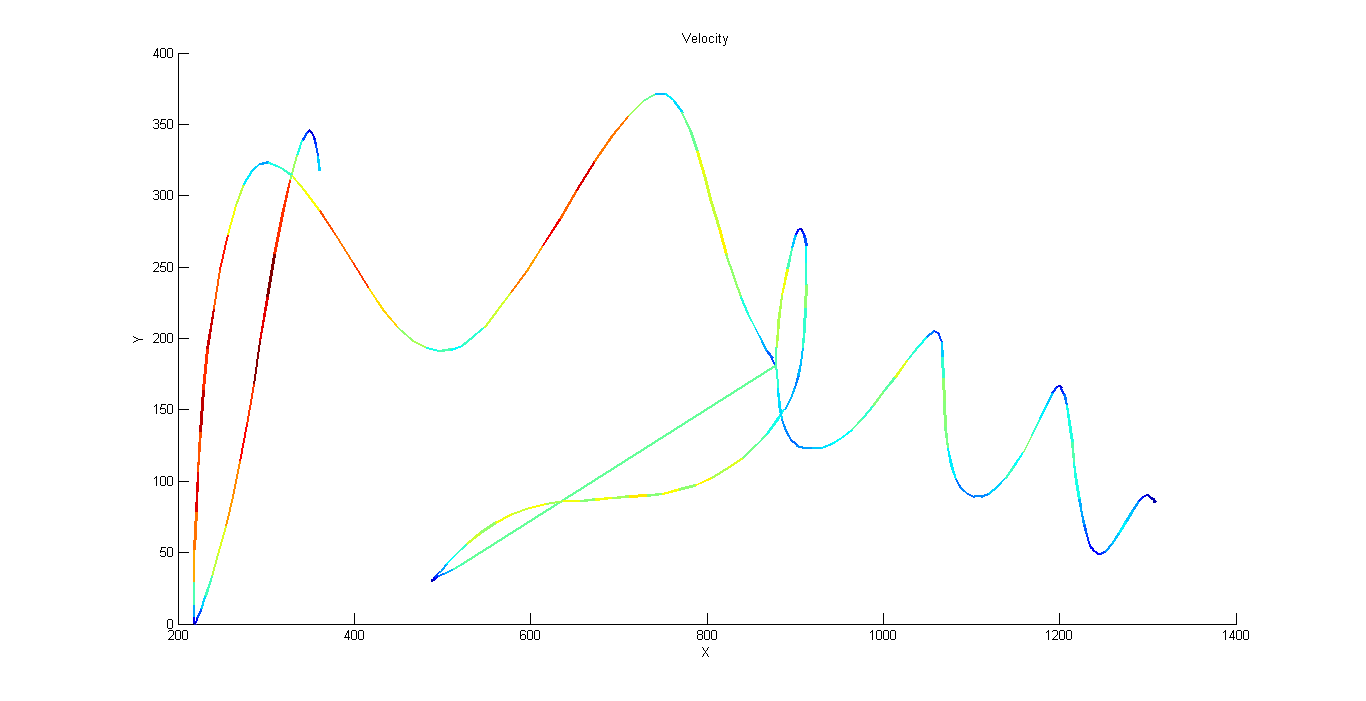
\includegraphics[width=0.5\linewidth]{MSigForge_Velocity.png}
    \caption{Example "Forged" Velocity Mapped Signatures Captured}
    \end{figure}
	% TODO - Screen Capture (Two Examples)
\item 3D Pressure Graph
	\subsubsection*{Real}
	\begin{figure}[H]
    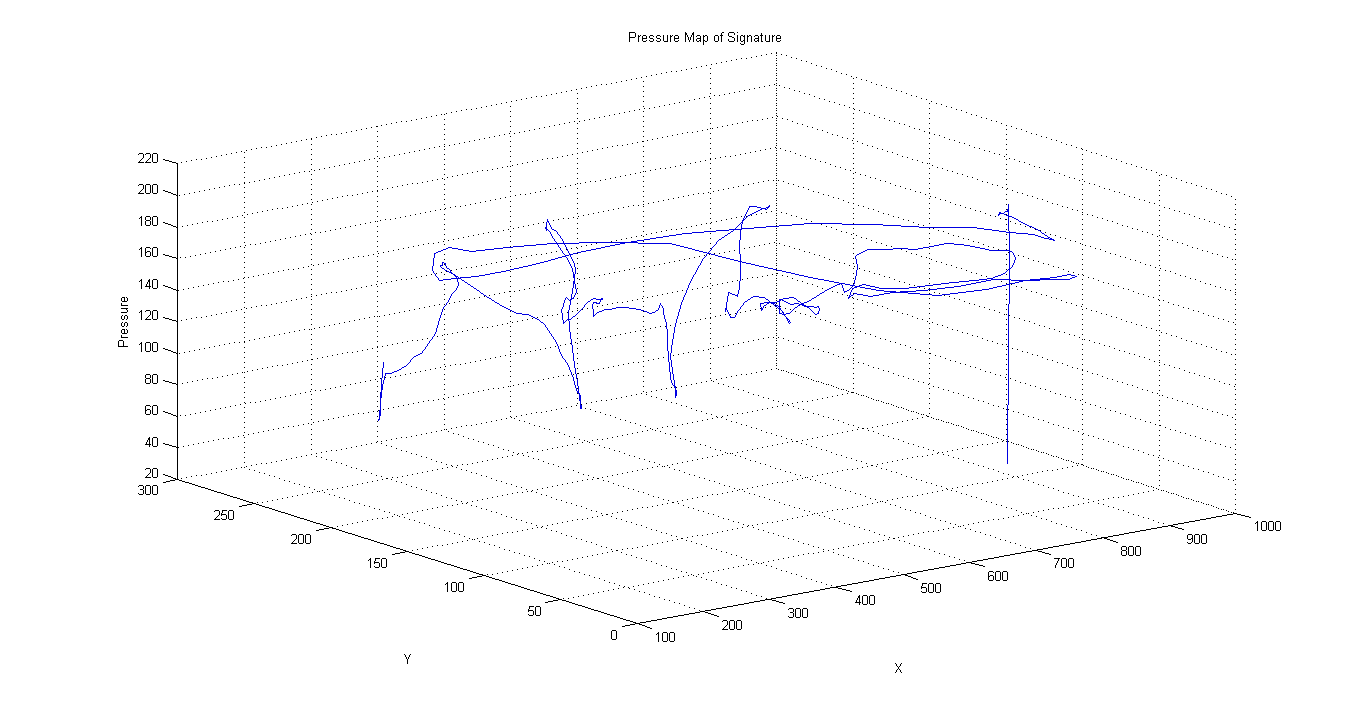
\includegraphics[width=0.5\linewidth]{KSig_Ex_Pressure3D.png}
    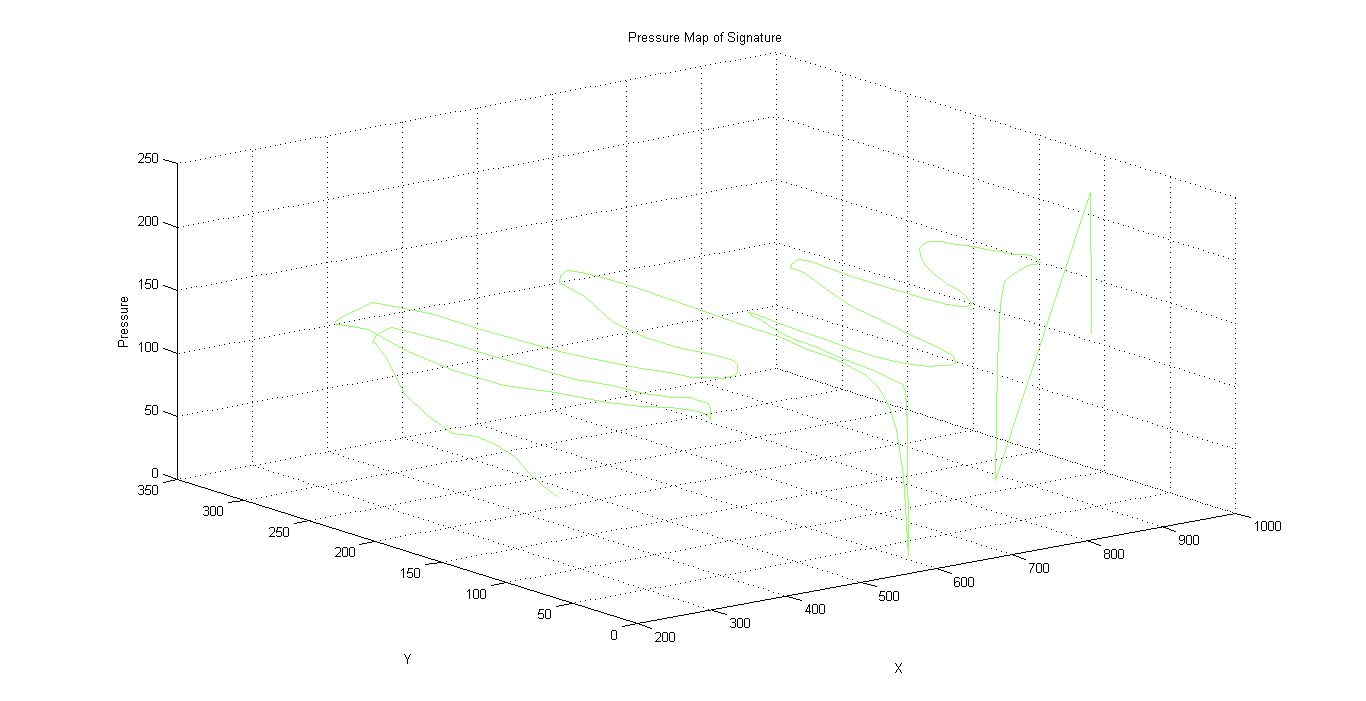
\includegraphics[width=0.5\linewidth]{MSig_Ex_Pressure3D.png}
    \caption{Example "Real" 3D Pressure Mapped Signatures Captured}
    \end{figure}
    \subsubsection*{Forged}
    \begin{figure}[H]
    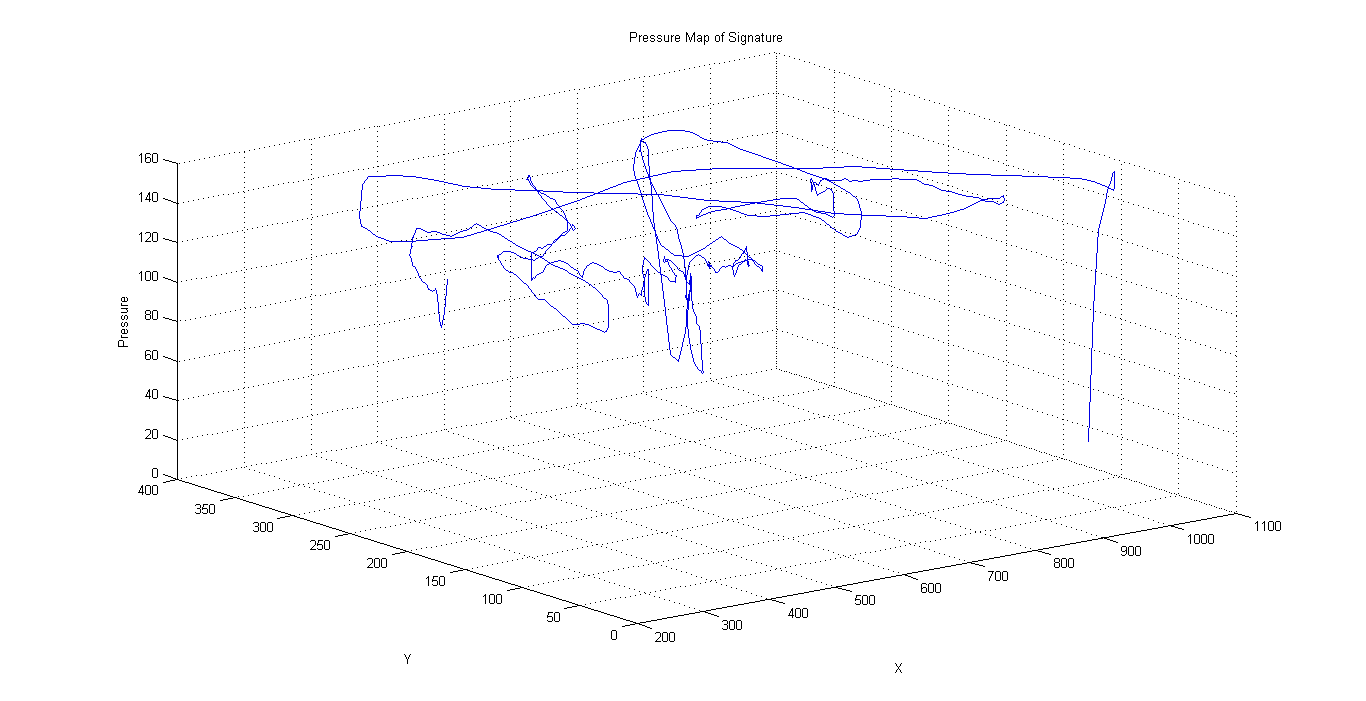
\includegraphics[width=0.5\linewidth]{KSigForge_Pressure3D.png}
    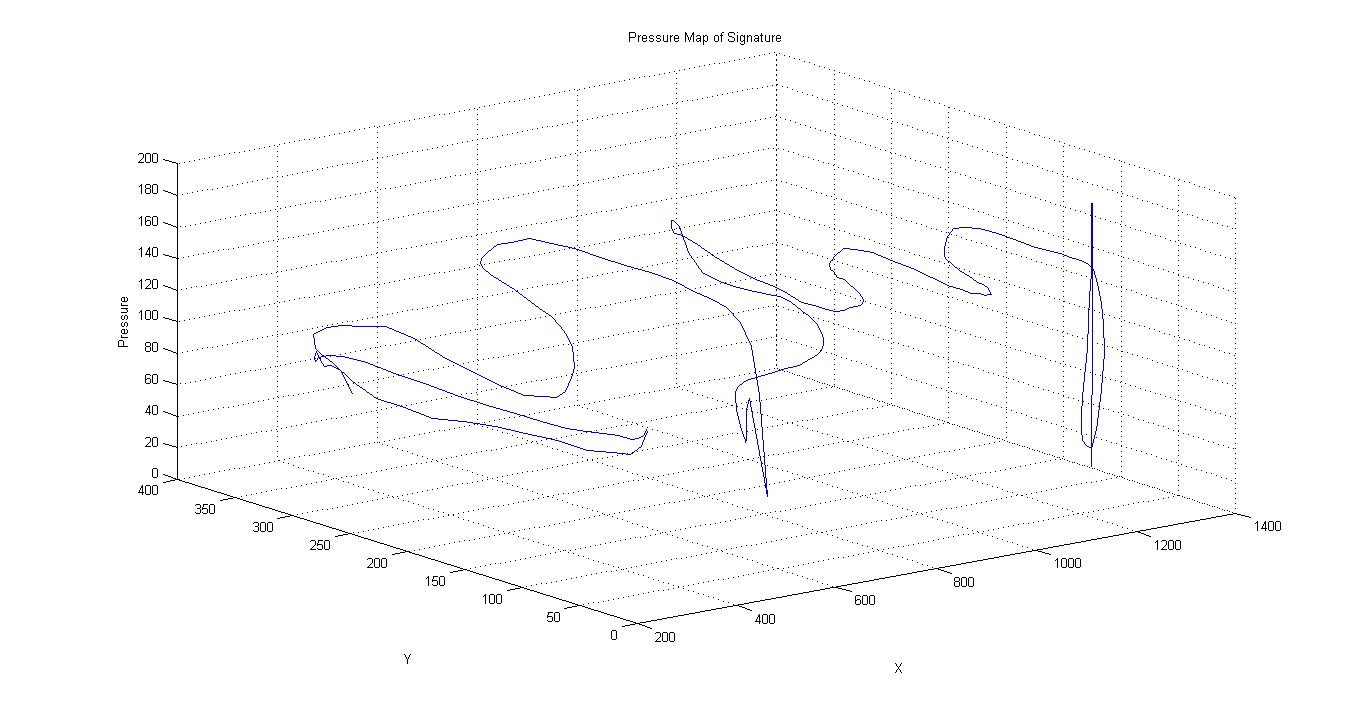
\includegraphics[width=0.5\linewidth]{MSigForge_Pressure3D.png}
    \caption{Example "Forged" 3D Pressure Mapped Signatures Captured}
    \end{figure}
	% TODO - Screen Capture (Two Examples)
\item Statistical Evaluation
	% TODO - Screen Capture (All Examples)
    \subsubsection*{Real}
    \begin{figure}[H]
    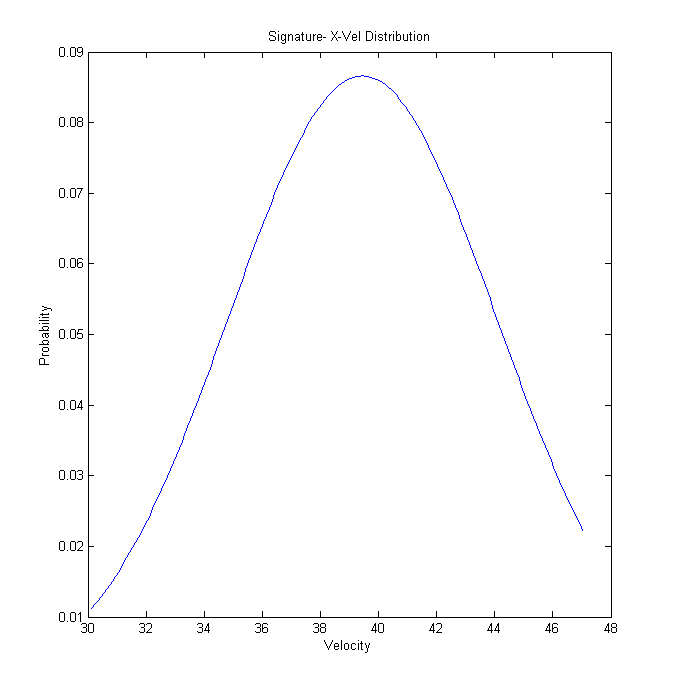
\includegraphics[width=0.5\linewidth]{KSig_X_Dist.png}
    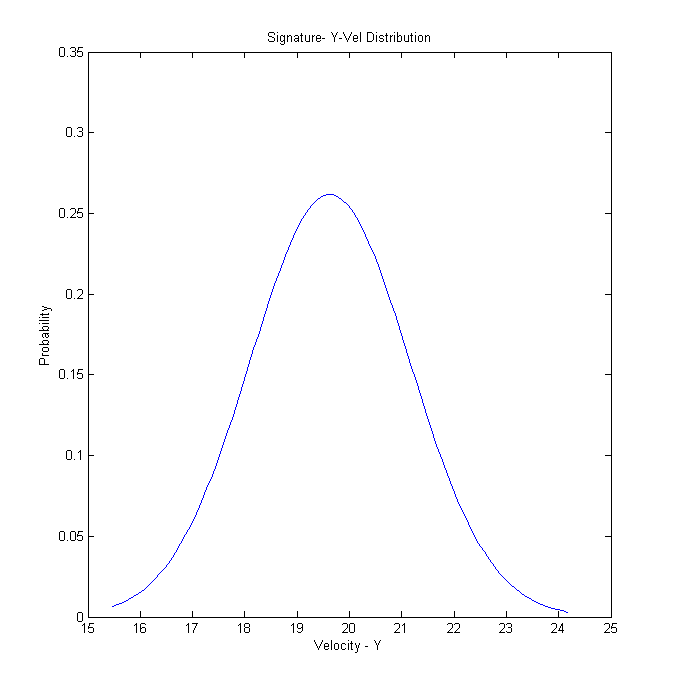
\includegraphics[width=0.5\linewidth]{KSig_Y_Dist.png}
    \caption{Example "Real" Statistical Distributions of K-Signature}
    \end{figure}
    \begin{figure}[H]
    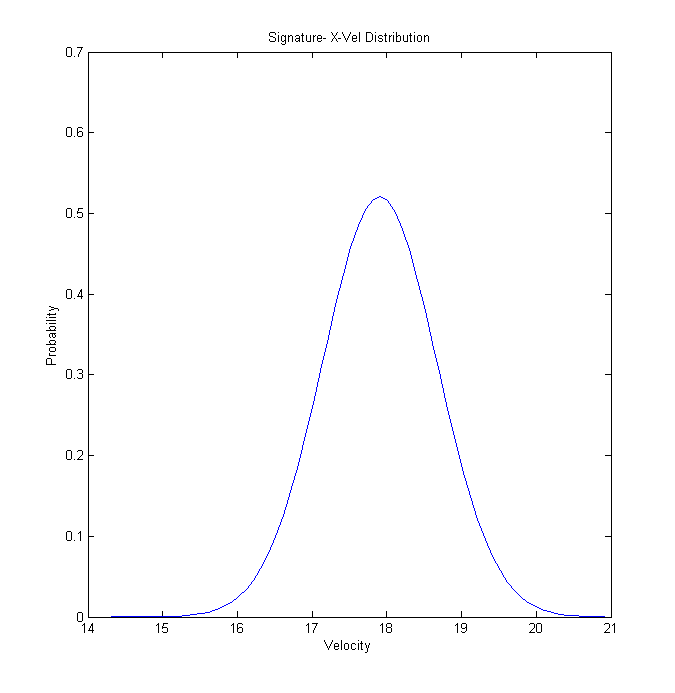
\includegraphics[width=0.5\linewidth]{MSig_X_Dist.png}
    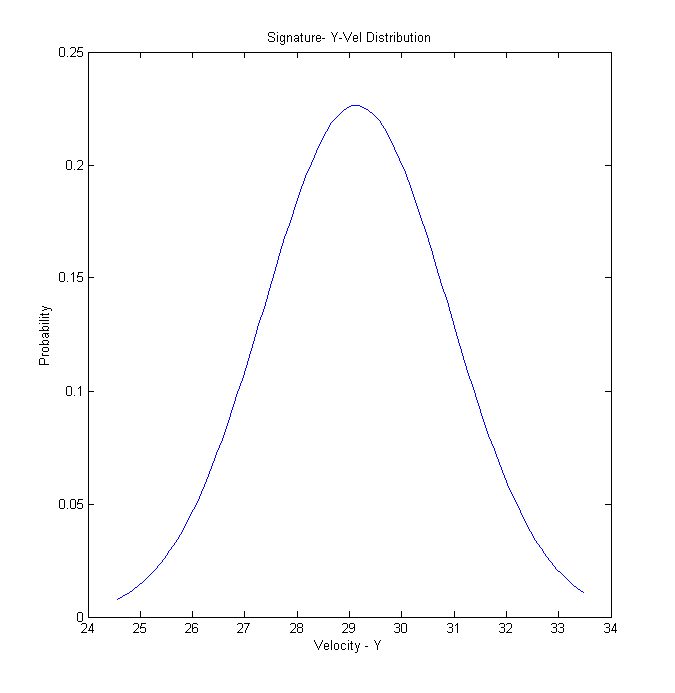
\includegraphics[width=0.5\linewidth]{MSig_Y_Dist.png}
    \caption{Example "Real" Statistical Distributions of M-Signature}
    \end{figure}
    \subsubsection*{Forged}
    \begin{figure}[H]
    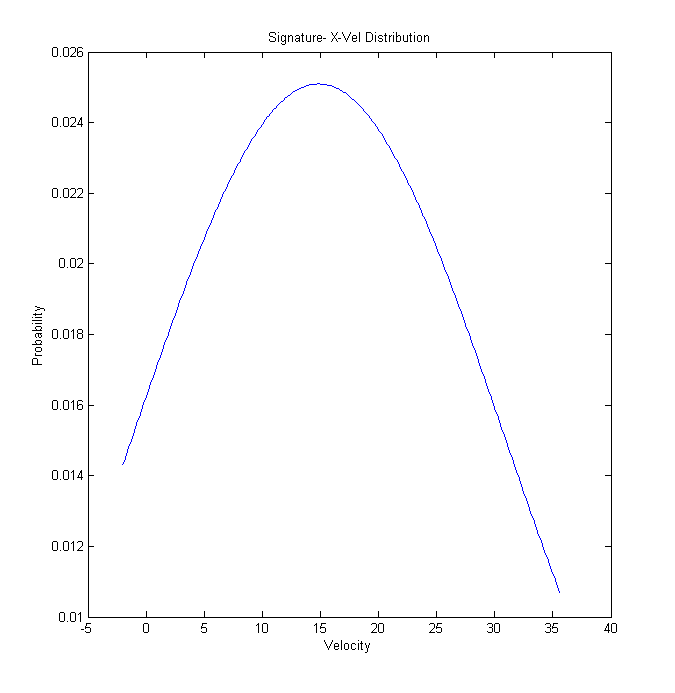
\includegraphics[width=0.5\linewidth]{KSigForge_X_Dist.png}
    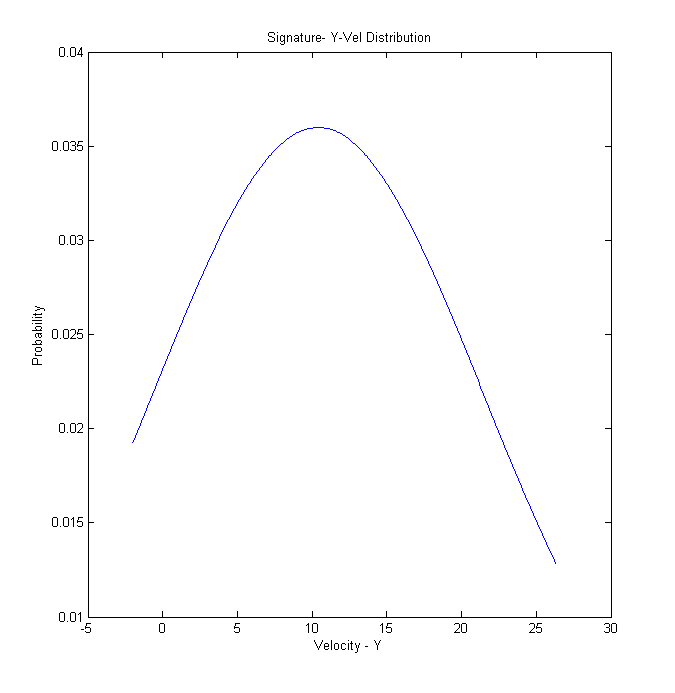
\includegraphics[width=0.5\linewidth]{KSigForge_Y_Dist.png}
    \caption{Example "Forged" Statistical Distributions of K-Signature}
    \end{figure}
    \begin{figure}[H]
    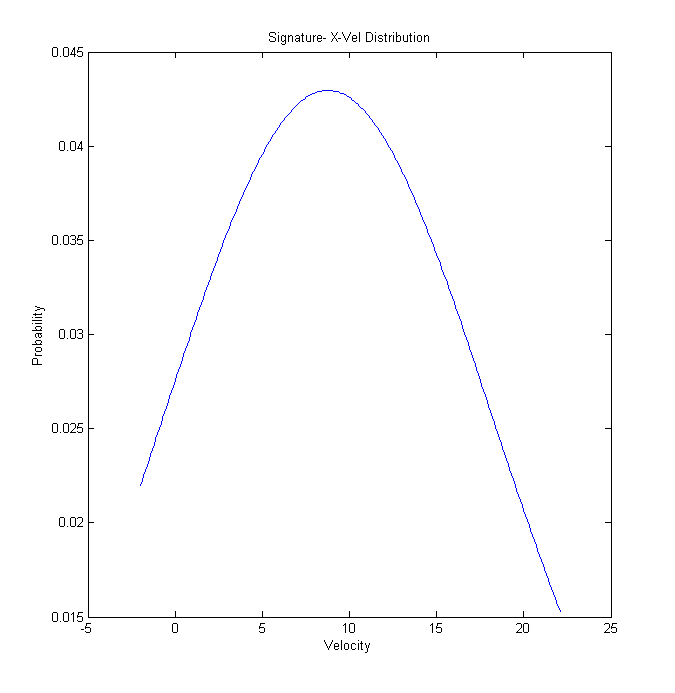
\includegraphics[width=0.5\linewidth]{MSigForge_X_Dist.png}
    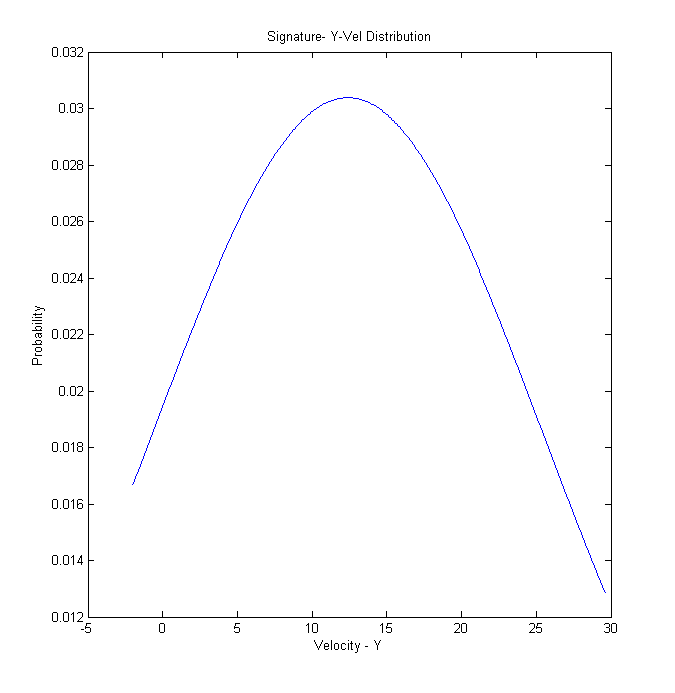
\includegraphics[width=0.5\linewidth]{MSigForge_Y_Dist.png}
    \caption{Example "Forged" Statistical Distributions of M-Signature}
    \end{figure}
\end{enumerate}

% DISCUSSION
\section{Discussion}
	\begin{itemize}
    \item \textbf{Problem 1 - Issue with Loss of Contact} \\ In order to correct for issues involving a loss of contact, we decided to throw in a conditional check via an If-Statement. Essentially, since MATLAB indexes its information starting with 1, we adjusted the pressure map index value to automatically search for \emph{one (1)} in the event of a \emph{zero (0)}.
    \item \textbf{Problem 2 - Issue with the colour bar} \\ During operation of the lab exercises, we as a group were unable to make MATLAB show its colour bars on any of the figures. This appears to be caused by some sort of path dependency issue as one solution online suggested it may be calling a different version of a built-in function which could be supplying the issue. That or the code needs to be updated to account for the newest features in MATLAB 2015a.
    \item \textbf{Statistical Distributions} \\ After performing an average of the velocity in both the X- and Y- directions, the distributions were analyzed and compared amongst each other. The comparison made apparent the vast difference in the statistical distributions of the different signatures and showcased variations in individual tendencies to write quickly in a particular direction. The distributions did in-fact resemble normal Gaussian distributions and as such our assumption was justified. 
    \item \textbf{Comparison between Real and Forged} \\ Between our two sets of "real" signatures, the distributions were very much different, and upon comparing them to their corresponding "forged" version, they too were also different. This goes to show that statistical analysis would be a sufficient method of comparing and contrasting whilst allowing for variations within the individual signature data.
    \end{itemize}
	% TODO - Enter in all required questions

% CONCLUSIONS
\section{Conclusion/Remarks on the Lab}
	The lab for the most part went off without any problems and the results were as expected. We did run into issues with the colour bars which we were unable to resolve however we did resolve the issue of indexing and loss of contact. Overall, the lab was quite simple and was a nice refresher for MATLAB as well as providing a good starting point into biometric analysis.
	% TODO - Enter in any Comments for the Lab and Final Conclusion of Exercise
\pagebreak
% MATLAB CODE
\section{Appendix A - MATLAB Code}
	% TODO - Enter in Matlab Code
\begin{MATLAB}
function Full_Lab1()
% function Full_Lab1()
%
%   Performs the Calculations for Lab 1 and calls on minor function
%
%   Authors:    Kyle MacInnis & Mebrhatom Anenya
%   Date:       September 16, 2015
%   Course:     ENCM 509
%

% Close all Windows
close all;

% Make Empty Arrays for velocity, Coords, and Pressure
xVelocity = zeros(1,10,'double');
yVelocity = zeros(1,10,'double');

% xPressure = zeros(1,10,'double');
% yPressure = zeros(1,10,'double');
%
% xCoords = zeros(1,10,'double');
% yCoords = zeros(1,10,'double');

% Load and fill Data from Signatures
for i = 1:5
    % Example Signatures
    %filename = strcat('sy',num2str(i),'.mat');
    
    % Real Signatures
    %filename = strcat('kSig',num2str(i),'.mat');
    %filename = strcat('msig',num2str(i),'.mat');
    
    %Forged Signatures
    filename = strcat('ksigf',num2str(i),'.mat');
    filename = strcat('msigf',num2str(i),'.mat');
    
    % load basic Signature Data
    [COORDi, TIMEi] = Lab1(filename,1);
    
    % Separate into X and Y data
    coordX = COORDi(:,1);
    coordY = COORDi(:,2);
    % Calculate Range of Data
    maxSize = max(size(COORDi,1))-1;
    % generate empty velocity vectors
    xVel = zeros(1,maxSize,'double');
    yVel = zeros(1,maxSize, 'double');
    % loop through data
    for j = 1:maxSize
        xDiff = abs(coordX(j+1) - coordX(j));
        yDiff = abs(coordY(j+1) - coordY(j));
        timeElapsed = double(TIMEi(j+1) - TIMEi(j));
        % Calculate Directional Velocities
        xVel(j) = (xDiff/timeElapsed)+1;
        yVel(j) = (yDiff/timeElapsed)+1;
    end
    
    % Calculate the average
    xVelAvg = 0;
    yVelAvg = 0;
    for j = 1:maxSize
        xVelAvg = xVelAvg + xVel(j);
        yVelAvg = yVelAvg + yVel(j);
    end
    xVelocity(i) = xVelAvg/maxSize;
    yVelocity(i) = yVelAvg/maxSize;
end
% Scale up Velocities
xVelocity = xVelocity * 10;
yVelocity = yVelocity * 10;

%% Perform Statistical Analysis on Data
% X- Direction
RangeX = min(xVelocity)-2:0.1:max(xVelocity)+2;
MeanX = mean(xVelocity);
StdX = std2(xVelocity);
ProbX = normpdf(RangeX,MeanX,StdX);
% Y-Direction
RangeY = min(yVelocity)-2:0.1:max(yVelocity)+2;
MeanY = mean(yVelocity);
StdY = std2(yVelocity);
ProbY = normpdf(RangeY,MeanY,StdY);

% plot Statistical Distribution
figure('name','X-Direction Normal Distribution');
plot(RangeX,ProbX);
xlabel('Velocity');
ylabel('Probability');
tname = strcat('Signature','- X-Vel Distribution');
title(tname);

figure('name','Y-Direction Normal Distribution');
plot(RangeY,ProbY);
xlabel('Velocity - Y')
ylabel('Probability');
tname = strcat('Signature','- Y-Vel Distribution');
title(tname);
\end{MATLAB}

\begin{MATLAB}
function [COORD, TIME] = Lab1(sigFile,n)
%% Lab 1 - Loads and Performs Analysis of Signatures
%
%   Authors:    Kyle MacInnis & Mebrhatom Anenya
%   Date:       September 16, 2015
%   Course:     ENCM 509
%
%
%   sigFile - filename (.mat file)
%   n - Display Figures or Not (For Full Lab File Run) (0 for figures)
%

% Close Figures
close all;

% Load in Signature Data
Sig1 = load(sigFile);
coord1 = double(Sig1.coord);
time1 = double(Sig1.time);
prs1 = double(Sig1.prs);

% return Time
TIME = time1;

% Reverse Direction of the Y Position (From Bottom Left)
coord1(:,2) = max(coord1(:,2)) - coord1(:,2);

% return Coordinates
COORD = coord1;

%% Plot 2D Signature Pressure
if n == 0
    figure('name','Signature - 1');
    pressureMap = colormap(jet(max(prs1)));
    % Connect Lines between each point
    for i = 1:(size(prs1,1)-1)
        
        if(prs1(i+1) == 0)
            prsMap = pressureMap(1,:);
        else
            prsMap = pressureMap(prs1(i+1),:);
        end
        line([coord1(i,1) coord1(i+1,1)], [coord1(i,2) coord1(i+1,2)], 'color', prsMap, 'linewidth', 2);
    end
    xlabel('X');
    ylabel('Y');
    title('Pen Pressure');
end

%% velocity Calculations
% Create Empty Vector
vel = zeros(size(time1,1)-1, 1);
for i = 1:size(time1,1)-1
    % Find Euclidean Distance
    distance = sqrt((coord1(i+1,1)-coord1(i,1))^2 + (coord1(i+1,2)-coord1(i,2))^2);
    vel(i) = distance/(time1(i+1) - time1(i));
    vel(i) = int32((vel(i)*1000)+1);
end
vel = [1; vel];

%% Plot Velocity Map in 2D
if n == 0
    velmap = colormap(jet(max(vel)));    
    figure('name', 'Velocity Map');
    for i = 1:size(coord1,1)-1
        vMap = velmap(vel(i+1),:);
        line([coord1(i,1) coord1(i+1,1)], [coord1(i,2) coord1(i+1,2)], 'color', vMap, 'linewidth', 2);
    end
    xlabel('X');
    ylabel('Y');
    title('Velocity');
end

%% Plot Pressure in 3D
if n == 0
    figure('name', '3D Pressure');
    plot3(coord1(:,1), coord1(:,2),prs1, 'color', prsMap);
    xlabel('X');
    ylabel('Y');
    zlabel('Pressure');
    title('Pressure Map of Signature');
    grid on;
end
\end{MATLAB}
\end{document}